\section{Simulation}

To simulate the dynamics of the mirror response, use MATLAB and generate random input disturbance vectors. The random disturbance, $\vec{D}$, is applied at the node \#2 (right) and given as Equation~\eqref{eq:dist}. The disturbance input is a force with random magnitude, $r$, and random direction, $\theta$, where $r \sim \mathcal{N}\left(r_0,\sigma_0\right)$ and $\theta \sim \mathcal{U}\left(0,2\pi\right)$. For this simulation, the input is an impulse at $t=0$, so the only non-zero value in the disturbance vector is at the initial state.\\

\begin{equation}
\label{eq:dist}
	\vec{D} = \left[
					\begin{array}{c}
					D_x\\
					D_y\\
					\end{array}
					\right]
				= \left[
					\begin{array}{c}
					r\cos{\theta}\\
					r\sin{\theta}\\
					\end{array}
					\right]
\end{equation}\\

 A first-order state-space representation of the equations of motion is integrated using \texttt{ODE45()} in MATLAB. Thus, for a realization of the random disturbance, a numerical deterministic solution of the mirror dynamics is obtained. The output is chosen to be the optical performance parameter of maximum spot size radius based on an exact raytrace. At each state, an exact raytrace as shown in a perturbed case by Figure~\ref{rt} is simulated in MATLAB using objects of \texttt{MirrorClass.m} and \texttt{RayClass.m}. In the focal plane, Figure~\ref{sd}, the maximum spot size radius is calculated as the euclidean norm of the chief ray intersection point with the intersection point of the ray farthest from the chief ray in the focal plane. The deviation of the chief ray intersection point from its nominal location is not considered. \\
 
 \begin{figure}	% rtsd
 \centering
 \subfigure[]{
 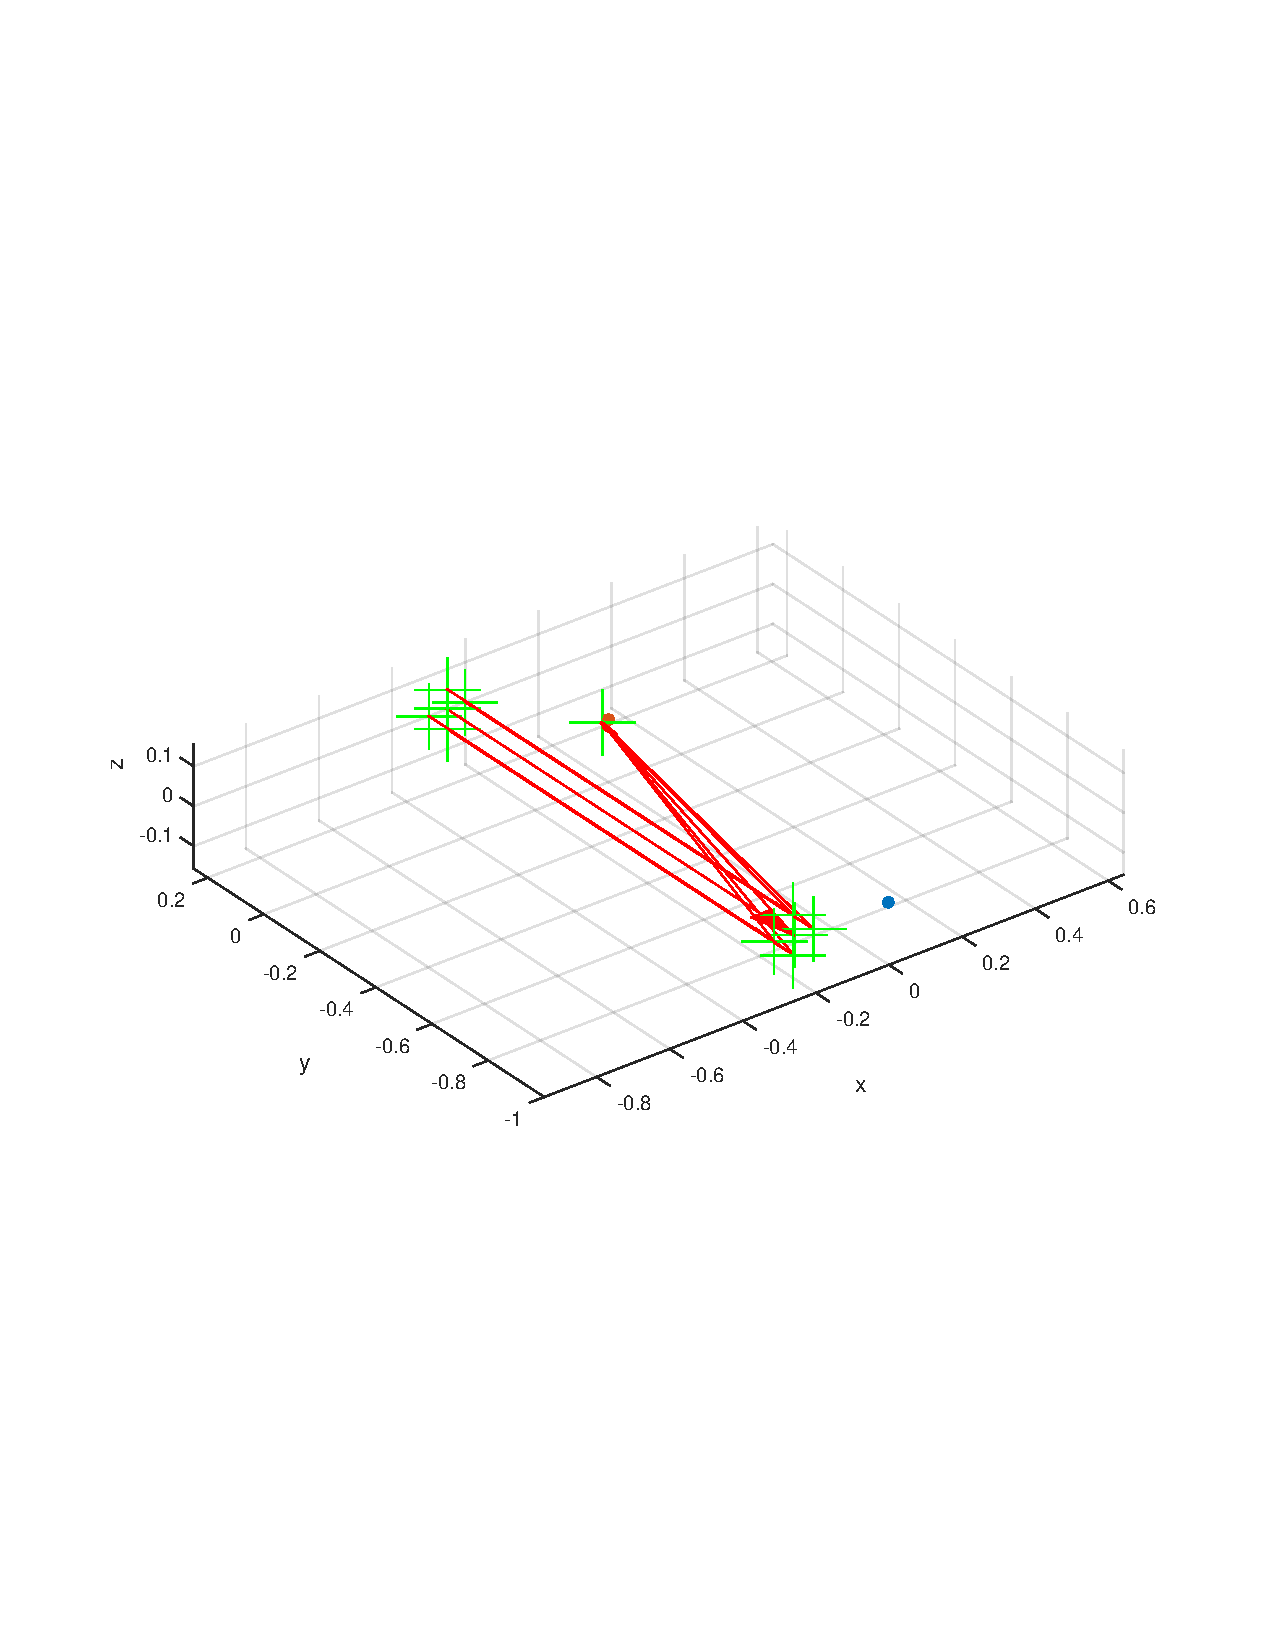
\includegraphics[width=0.45\textwidth,trim=1cm 6cm 2cm 6cm,clip]{Figures/Q5P1_raytrace.pdf}
 \label{rt}}
 \subfigure[]{
 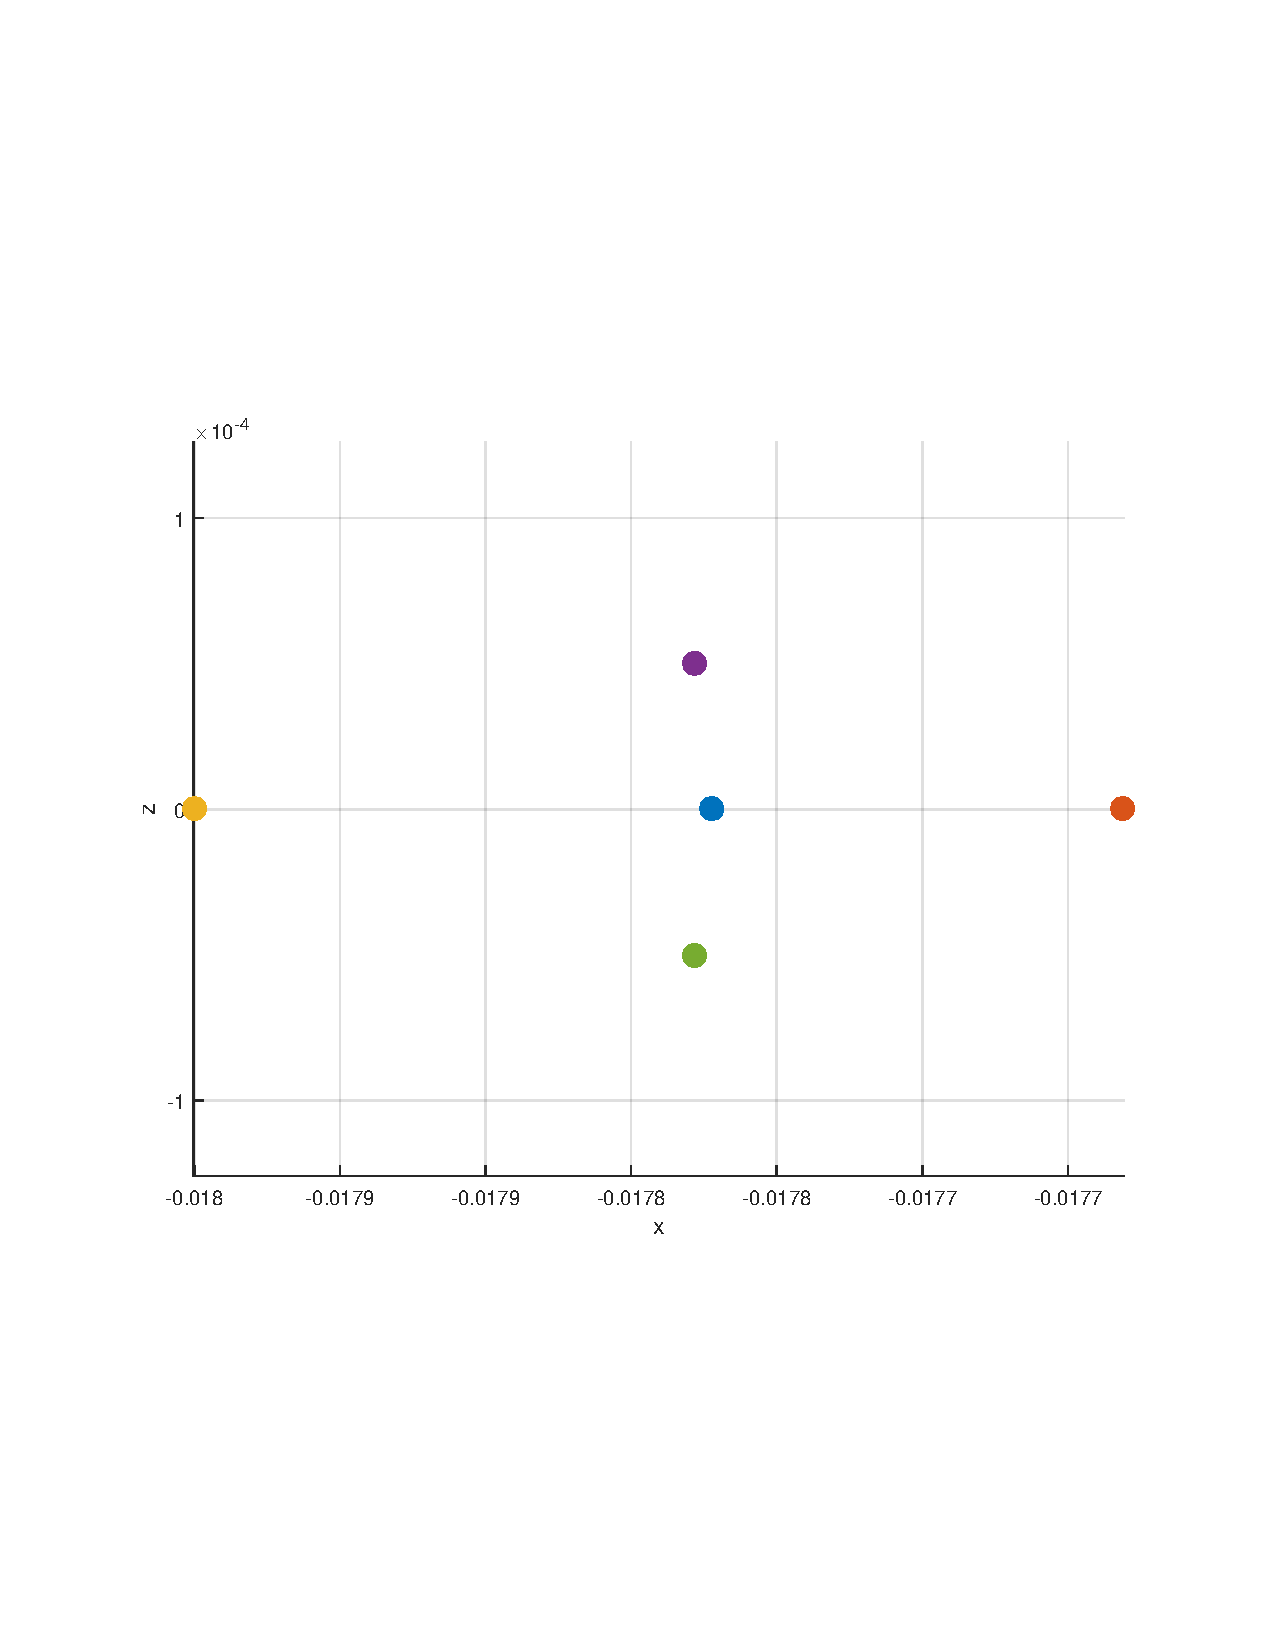
\includegraphics[width=0.45\textwidth,trim=1cm 6cm 2cm 6cm,clip]{Figures/Q5P1_spotdiagram.pdf}
 \label{sd}}
 \caption{Raytrace (a) and corresponding detector plane spot diagram (b) for mirror in a perturbed state (rotation about the z-axis).}
 \label{rtsd}
\end{figure}
 
 When a Monte Carlo Simulation is run, a complete state history of the input and output are available for each realization and each combination of disturbance distribution parameters, $r_0$ and $\sigma_0$. The cost functional of each realization is the average of the maximum spot size radius at each state. A Gaussian distribution is assumed for the scalar output performance measure and the mean and standard deviation of this average are calculated for all realizations of a given distribution (i.e.\ $r_{ss_{max}} \sim \mathcal{N}\left(\mu_{out},\sigma_{out}\right)$ given $r_0$ and $\theta_0$). Thus, the output distribution parameters, $\mu_{out}$ and $\sigma_{out}$, are generated as a function of the input disturbance distribution parameters, $r_0$ and $\theta_0$.\\
 
 \subsection*{MATLAB Simulation Details}

\begin{sloppypar} 
The MATLAB simulation script first defines the geometric properties of the system. The function, \texttt{calcConicCentroid.m}, returns the indices of the centroid, point 1, and point 2 as well as the mass and moment of inertia of the parabolic mirror segment. Next, values are assigned to the spring rate and damping coefficient and the simulation time is specified. The MCS is accomplished by generating sample realizations of the disturbances, simulating mirror dynamics, and calculating the corresponding optical outputs a number of times for each disturbance distribution. Function \texttt{Q5\_Realization.m} returns the output dynamics and the spotsize for a given $r_0$ and $\sigma_0$, then the mean and standard deviation is computed for each combination. \\
 \end{sloppypar}
 
The function \texttt{Q5\_Realization.m} generates the random impulse disturbance based on the supplied distribution parameters. Function \texttt{state\_eqns.m} is supplied the time span, initial guess, and disturbance vector and the deterministic solution is computed by numerical integration of the first-order state equations using \texttt{ODE45.m}.From the output state vector, the mirror vertex position is calculated. The change in vertex position from the nominal location as well as the perturbed angle is passed to function \texttt{SingleMirror\_SpotSize.m}.\\
 
\texttt{SingleMirror\_SpotSize.m} defines properties of the mirror conic section and the direction of the input beam. Mirror objects are constructed from \texttt{MirrorClass.m} with the mirror properties and these mirror objects are used to construct ray objects from \texttt{RayClass.m}. Each ray object can be thought of as one complete trace of a ray through the optical system. It contains a segment for each propagation step and the coordinates of each endpoint of each segment. The class files \texttt{MirrorClass.m} and \texttt{RayClass.m} utilize and compliment work presented by Breckenridge and Redding.~\cite{RedBreck} The final surface in the raytrace is the reference surface and the intersection point of the rays with that plane defines the spot diagram. \texttt{SingleMirror\_SpotSize.m} finishes by calculating the distance between the chief ray and each of the marginal ray reference surface intersection points and determines the maximum distance. This maximum distance is defined as the spot size for this analysis.After all realizations have run and the distribution of the output has been calculated, the results are plotted.
